\section{Progettazione di un Data Mart}
Gli attori che partecipano a questa fase sono il Progettista, l'Amministratore del DB e l'utente finale.
La realizzazione di un Data Mart avviene seguendo determinate fasi:
\begin{enumerate}
	\item \textbf{Analisi e Riconciliazione delle Sorgenti}: Si esaminano tutti i DB che dovranno essere utilizzati dal Data Mart, normalizzare ed integrare ciò che non lo è. In questa fase sostanzialmente viene progettato l'ODS.
	\item \textbf{Analisi dei requisiti}: Interviste agli utenti finali, si capisce quali sono i requisiti necessari.
	\item \textbf{Progettazione Concettuale}: Si disegna lo schema concettuale del Data Mart sulla base dei requisiti utente e dei dati presenti nello schema riconciliato.
	\item \textbf{Carico di Lavoro e Volume dati}: Analisi delle Query che verranno utilizzate di più nel Data Mart. Si capisce il volume dei dati.
	\item \textbf{Progettazione Logica}: Viene creato lo schema logico (relazionale).
	\item \textbf{Progettazione dell'ETL}: Si progettano le procedure ETL sulla base degli schemi sorgente, dello schema riconciliato, e dello schema logico del Data Mart.
	\item \textbf{Progettazione Fisica}: Schelta degli indici e di altri aspetti secondari.
	\item \textbf{Implementazione della Reportistica}: Creazione dei report a partire dai dati.
	\item \textbf{Testing}: Si potrebbero testare diversi aspetti di quanto già riportato, ma la parte più importante da testare è l'ETL.
\end{enumerate}
La fase che in genere occupa circa il 70\% dell'effort del progetto è la progettazione dell'ETL. Le procedure di pulizia e trasformazione sono infatti estremamente specifiche e legate ai dati dell'azienda, e quindi difficilmente generalizzabili.

\subsection{Quadro metodologico}
Esistono due grandi scenari possibili quando si effettua la progettazione di Data Mart, l'approccio guidato dai dati (data-driven o supply-driven) e quello guidato dai requisiti (demand-driven).

\subsubsection{Approccio guidato dai dati}
Il Data Mart viene progettato a seguito di una attenta analisi delle sorgenti operazionali. I requisiti utente impattano sul progetto guidando il progettista nella selezioni delle porzioni di dati considerate.\newline
Esiste un algoritmo che a partire dallo schema dei DB sorgenti si può arrivare allo schema concettuale del Data Mart in modo molto semplice ed automatico.
\begin{info}[Parallelismo con il mondo reale:]
	Se ho fame e torno a casa, guardo cosa ho nel frigo e uso ciò che ho, anche se magari non è esattamente ciò che mi piace.
\end{info}

\begin{itemize}
	\item Avendo a disposizione gli schemi logici dei DB sorgente li esamino e li studio. Effettuo una \textbf{Analisi e Riconciliazione}, ottenendo così lo schema riconciliato (ODS).
	\item Avendo a disposizione lo schema riconciliato, parte l'analisi dei requisiti, da cui si ottiene un glossario di richieste di utenti e note. Segue la \textbf{Progettazione Concettuale} che in output restituisce lo schema di fatto.
	\item A seguito del Raffinamento del carico di lavoro si effettua la \textbf{Progettazione Logica} a partire dallo schema di fatto.
	\item A questo punto di può cominciare a \textbf{progettare l'ETL}. Si ottiene quindi lo schema dell'alimentazione.
\end{itemize}
\begin{itemize}
	\item \textbf{VANTAGGI}:
	\begin{itemize}
		\item Lo schema concettuale di massima si deriva algoritmicamente.
		\item Progettazione dell'ETL risulta notevolmente semplificata, ciascuna informazione del Data Mart è associata direttamente a uno o più attributi della sorgente, necessariamente.
	\end{itemize}

	\item\textbf{SVANTAGGI}:
	\begin{itemize}
		\item Requisiti utenti vengono meno, hanno un ruolo secondario.
		\item Supporto limitato al progettista per l'identificazione di fatti dimensioni e misure.
	\end{itemize}
\end{itemize}
\noindent Questo approccio non sempre è applicabile, lo è quando:
\begin{itemize}
	\item Sono disponibili o ottenibili con costo contenuto gli schemi delle sorgenti.
	\item Gli schemi sorgenti hanno un buon grado di normalizzazione.
	\item La complessità degli schemi sorgenti non è eccessiva.
\end{itemize}
\noindent Un ottimo punto di partenza è l'ODS, infatti tutti i requisiti sono garantiti se l'ODS esiste. Un altro caso valido è quello in cui esiste una sola sorgente ben progettata.

\begin{figure}[H]
	\begin{center}
		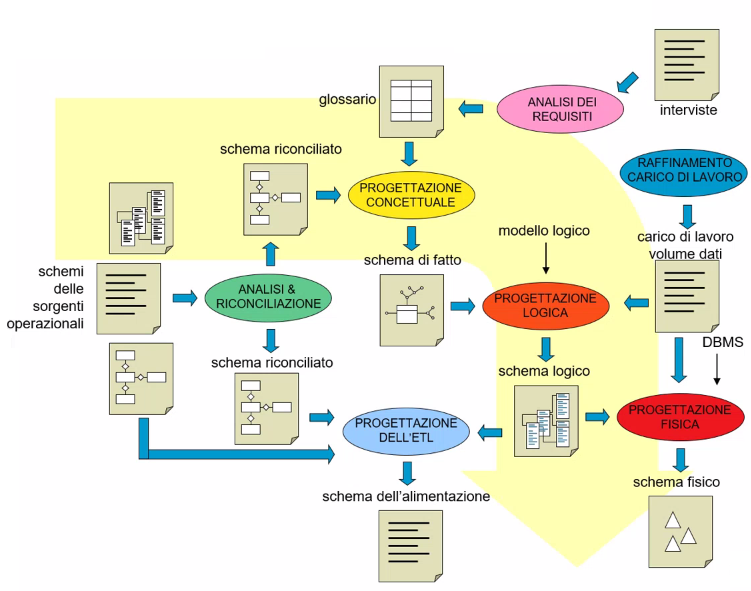
\includegraphics[width=0.8\linewidth]{img/data_approach.png}
		\caption{Approccio guidato dai dati.}
	\end{center}
\end{figure}

\subsubsection{Approccio guidato dai requisiti}
Si inizia determinando i requisiti informativi degli utenti del Data Mart. Il problema di come mappare i requisiti e le sorgenti dati vengono affrontati in seguito, non sono primari.\newline
Progettare il Data Mart è molto più difficile e non esiste un algoritmo. Anche progettare l'ETL è molto più difficile.
\begin{info}[Parallelismo con il mondo reale:]
	Ho fame e torno a casa, ho una gran voglia di carbonara. Parto con le aspettative di ottenerne una. Il rischio è che aprendo il frigo io mi accorga di non avere le uova.
\end{info}

\begin{itemize}
	\item Si parte dall'\textbf{Analisi dei Requisiti}.
	\item Segue la \textbf{Progettazione Concettuale}, da cui si ottiene lo schema di fatto.
	\item Si passa direttamente alla \textbf{Progettazione logica}, ottenendo lo schema logico.
	\item A questo punto è necessario progettare l'ETL, ma fino ad ora le sorgenti non sono mai state prese in considerazione, quindi la progettazione sarà più lunga e complessa.
	\item Segue la \textbf{Progettazione Fisica}.
\end{itemize}

\begin{itemize}
	\item \textbf{VANTAGGI}:
	\begin{itemize}
		\item I desideri dell'utente sono in primo piano.
	\end{itemize}
	\item \textbf{SVANTAGGI}:
	\begin{itemize}
		\item Progettazione dell'ETL costosa e complessa.
		\item I fatti, le gerarchie e le misure vengono dedotte dagli utenti. Solo a posteriori si viene a scoprire se ci sono inconsistenze tra le richieste e i dati effettivi.
		\item La fiducia del cliente verso il progettista e verso l'utilità del Data Mart può venir meno.
	\end{itemize}
\end{itemize}
\noindent Questo approccio è l'unica alternativa nei casi in cui non sia fattibile a priori un'analisi approfondita delle sorgenti, quando per esempio il Data Mart è alimentato da un ERP.

\begin{figure}[H]
	\begin{center}
		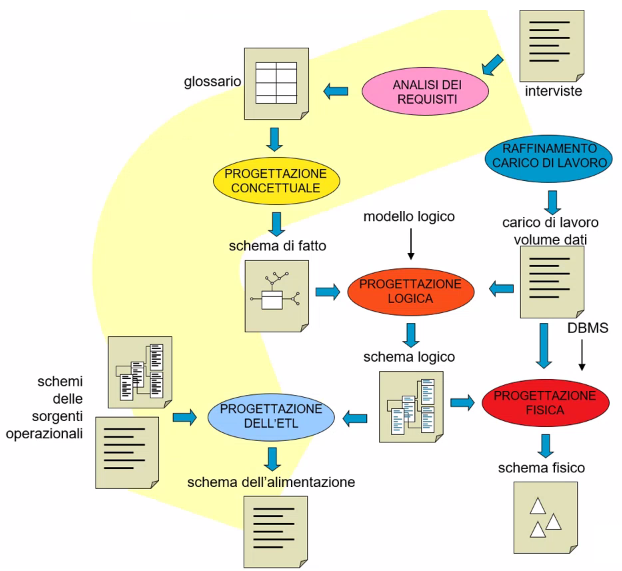
\includegraphics[width=0.6\linewidth]{img/req_approach.png}
		\caption{Approccio guidato dai requisiti.}
	\end{center}
\end{figure}
